\section{Natural Neighbor Coordinates\label{sec:coordinates}}
\subsection{Introduction}
Natural neighbor interpolation has been introduced by Sibson
\cite{s-bdnni-81} to interpolate multivariate scattered data.  Given
a set of data points $\mathcal{P}$, the natural neighbor coordinates
associated to $\mathcal{P}$ are defined from the Voronoi diagram of
$\mathcal{P}$.  When simulating the insertion of a query point
$\mathbf{x}$ into the Voronoi diagram of $\mathcal{P}$, the potential
Voronoi cell of $\mathbf{x}$ ``steals'' some parts from the existing
cells. 

\begin{figure}[ht!]
\begin{ccTexOnly}
\begin{center}
  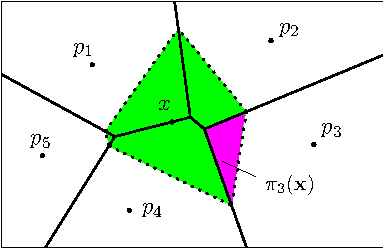
\includegraphics{Interpolation/nn_coords}
\end{center}
\end{ccTexOnly}

\begin{ccHtmlOnly}
<img border=0 src="./nn_coords.gif"  align=center  alt="nn_coords">
\end{ccHtmlOnly}

\caption{$2D$ example: $\mathbf{x}$ has five natural neighbors 
  $\mathbf{p_1},\ldots , \mathbf{p_5}$. 
  The natural neighbor coordinate $\lambda_3(\mathbf{x})$ is the ratio
  of the area of the pink polygon, $\pi_3(\mathbf{x})$, over the area
  of the total highlighted zone.
  \label{fig:nn_coords}}
\end{figure}



Let $\pi(\mathbf{x})$ denote the volume of the potential Voronoi cell
of $\mathbf{x}$ and $\pi_i(\mathbf{x})$ denote the volume of the
sub-cell that would be stolen from the cell of $\mathbf{p_i}$ by the
cell of $\mathbf{x}$.  The natural neighbor coordinate of $\mathbf{x}$
with respect to the data point $\mathbf{p_i}\in \mathcal{P}$ is defined by
$$
\lambda_i(\mathbf{x}) =
\frac{\pi_i(\mathbf{x})}{\pi(\mathbf{x})}.$$
A two-dimensional example
is depicted in Figure \ref{fig:nn_coords}.


Various papers (\cite{s-vidt-80}, \cite{f-sodt-90},
\cite{cgal:p-plcbd-93}, \cite{b-scaps-97}, \cite{hs-vbihc-00}) show that
the natural neighbor coordinates have the following properties:
  \begin{itemize}
  \item[(i)] $\mathbf{x} = \sum_{i=1}^n \lambda_i(\mathbf{x}) \mathbf{p_i}$
    (barycentric coordinate property).
  \item[(ii)] For any $i,j \leq n, \lambda_i(\mathbf{p_j})=
    \delta_{ij}$, where $\delta_{ij}$ is the Kronecker symbol.
  \item[(iii)] $\sum_{i=1}^n \lambda_i(\mathbf{x}) = 1$ (partition of unity
    property).
  \end{itemize}
  Furthermore, Piper \cite{cgal:p-plcbd-93} shows that the coordinate
  functions are continuous in the convex hull of $\mathcal{P}$ and
  continuously differentiable except on the data points $\mathcal{P}$.
  \medskip
  
  The interpolation package of \cgal\ provides functions to compute
  natural neighbor coordinates for $2D$ and $3D$ points with respect
  to Voronoi diagrams as well as with respect to power diagrams (only
  $2D$), i.e.\ for weighted points. Refer to the reference pages
  \ccc{natural_neighbor_coordinates_2},
  \ccc{natural_neighbor_coordinates_3} and
  \ccc{regular_neighbor_coordinates_2}.
  
  In addition, the package provides functions to compute natural
  neighbor coordinates on well sampled point set surfaces. See
  Section~\ref{sec:surface} and the reference page
  \ccc{surface_neighbor_coordinates_3} for further information.

\subsection{Implementation}
Given a Delaunay triangulation or a Regular triangulation, the
vertices in conflict with the query point are determined. The areas
$\pi_i(\mathbf{x})$ are computed by triangulating the Voronoi
sub-cells.  The normalization factor $\pi(\mathbf{x})$ is also
returned. If the query point is already located and/or the boundary
edges of the conflict zone are already determined, alternative
functions allow to avoid the re-computation.

\subsection{Example}
The signature of all coordinate computation functions is about the
same.
\ccIncludeExampleCode{Interpolation/nn_coordinates_2.C}
\subsubsection{Regular neighbor coordinate computation}
For regular neighbor coordinates, it is sufficient to replace the name
of the function and the type of triangulation passed as parameter. A
special traits class is needed.
\ccIncludeExampleCode{Interpolation/rn_coordinates_2.C}
For surface neighbor coordinates, the surface normal at the query
point must be provided, see Section~\ref{sec:surface}.
%
